%!TEX root =../../../course-notes.tex
% ^ leave for LaTeXTools build functionality

\begin{applicationActivities}




\begin{activity}{5}
Why don't clouds fall out of the sky?
\begin{center}
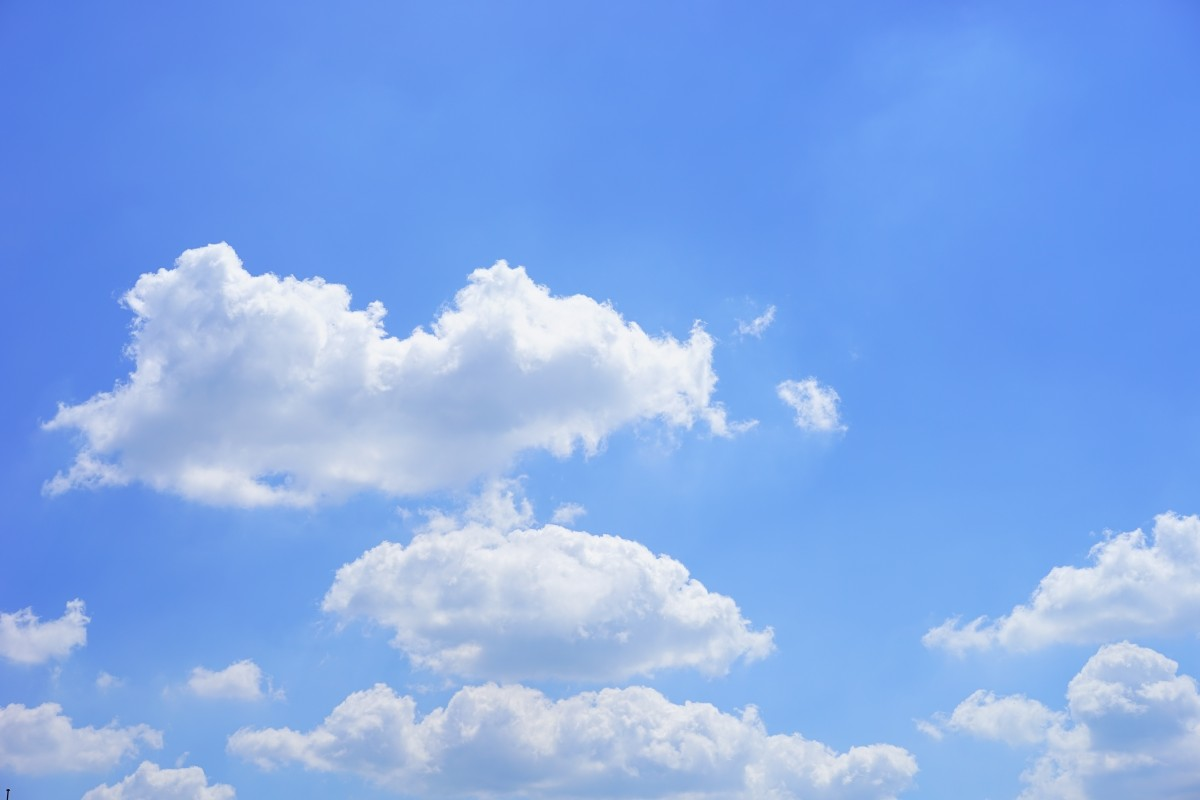
\includegraphics[scale=0.2]{media/cloud.jpg}
\end{center}

\begin{enumerate}[(a)]
\item They are lighter than air
\item Wind keeps them from falling
\item Electorstatic charge
\item They do fall, just very slowly
\end{enumerate}
\end{activity}

\begin{activity}{5}
List all of the forces acting on a tiny droplet of water falling from the sky.
\end{activity}

\begin{activity}{5}
Tiny droplets of water obey \term{Hook's law}, which says that air resistance is proportional to velocity.
\\~\\
Use Newton's laws to write a differential equation that models the velocity of a falling droplet of water.  
\end{activity}


\begin{definition}
A \term{first order constant coefficient} differential equation can be written in the form
\[y^\prime+by=c,\]
or equivalently,
\[\frac{dy}{dx} +by=c.\]
We will use both notations interchangeably.

Here, \term{first order} refers to the fact that the highest derivative we see is the first derivative of \(y\).
\end{definition}

\begin{observation}
Consider the differential equation \(y'=y\).

A useful way to visualize a first order differential equation is by a \term{slope field}


\begin{center}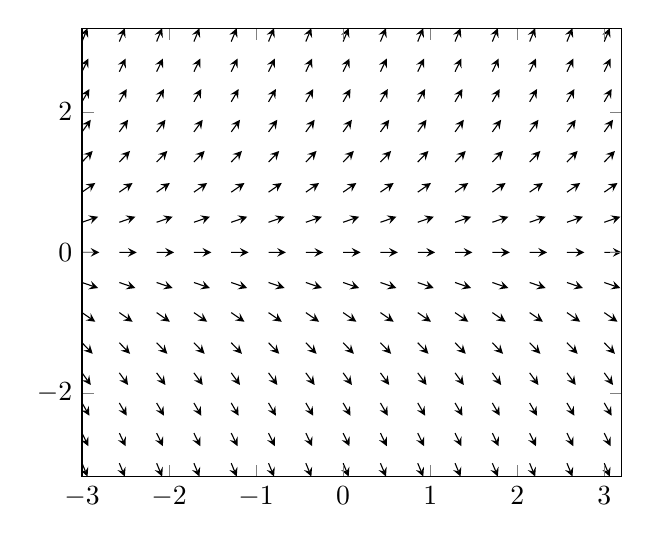
\begin{tikzpicture}
    \begin{axis}[
        domain=-3:3,
        view={0}{90},
        axis background/.style={fill=white},
    ]
        \addplot3[black,
            quiver={
             u={1/(sqrt(1 + (y)^2))},
             v={(y)/(sqrt(1 + (y)^2))},
             scale arrows=0.2,
            },
            -stealth,samples=15]
                {exp(-x) - 1/2*sin(x) - 1/2*cos(x)};
        %%KAWWWWWWW
        %% Here be some points added to the swoopy loop vector fieldamagigs
        %\addplot[mark=*] coordinates {(-1,2)}; % Obvious ordered pair for lococation
        %\addplot[mark=*] coordinates {(-1,-2)};
    \end{axis}
\end{tikzpicture}\end{center}
Each arrow represents the slope of a solution \term{trajectory} through that point.
\end{observation}

\begin{activity}{5}
Consider the differential equation \(y'=y\) with slope field below.

\begin{center}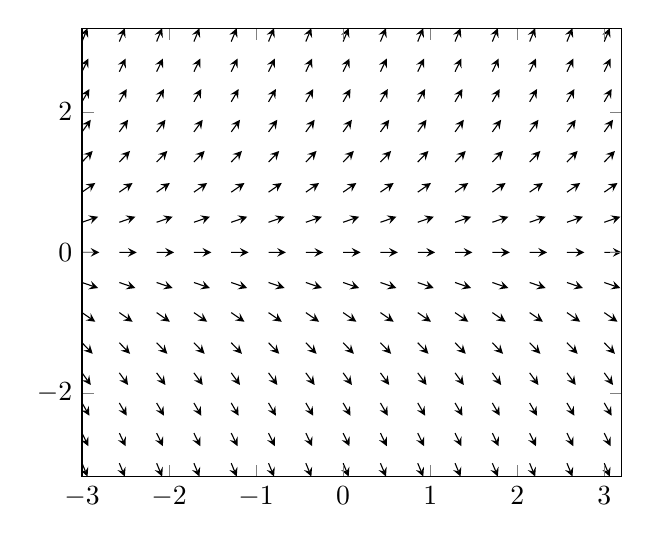
\begin{tikzpicture}
    \begin{axis}[
        domain=-3:3,
        view={0}{90},
        axis background/.style={fill=white},
    ]
        \addplot3[black,
            quiver={
             u={1/(sqrt(1 + (y)^2))},
             v={(y)/(sqrt(1 + (y)^2))},
             scale arrows=0.2,
            },
            -stealth,samples=15]
                {exp(-x) - 1/2*sin(x) - 1/2*cos(x)};
     \end{axis}
\end{tikzpicture}\end{center}
\begin{subactivity}
Draw a trajectory through the point \((0,1)\).
\end{subactivity}
\begin{subactivity}
Draw a trajectory through the point \((-1,-1)\).
\end{subactivity}
\end{activity}


\begin{activity}{15}
Consider the differential equation \(y^\prime=y\).
\begin{subactivity}
Find a solution to \(y^{\prime}=y\).
\end{subactivity}
\begin{subactivity}
Find {\bf all} solutions to \(y^{\prime}=y\).
\end{subactivity}
\end{activity}

\begin{definition}
A differential equation will have many solutions.  The \term{general solution} encompasses all of these by using 
parameters such as \(C,k,c_0,c_1\) and so on. For example:

\begin{itemize}
\item The general solution to the differential equation \(y'=2x-3\) is \(y=x^2-3x+C\) (as done in
Calculus courses).
\item The general solution for \(y'=y\) is \(y=c_0 e^x\) (as done in the previous activity). 
\end{itemize}

\end{definition}


\begin{activity}{15}
Adapt the solution \(y=c_0e^x\) for \(y^\prime=y\) to find a general solutions for
the following differential equations.
\begin{subactivity}
Solve \(y^{\prime}=2y\).
\end{subactivity}
\begin{subactivity}
Solve \(y^{\prime}=y+2\).
\end{subactivity}
\end{activity}

\end{applicationActivities}
